%% ID: maximum_deflection_angle
%% TITLE: Maximum Deflection of a Particle
%% TYPE: question
%% QUESTIONTYPE: numeric
%% CONCEPTS:  energy, momentum, zero_momentum_frame, vectors1, vectors2
%% VIDEOS: 
%% LEVEL: 6
%% TOPIC: mechanics/dynamics
%% ORDER: 8

\begin{problem}[Maximum Deflection of a Particle]   % suvat, force = rate of change in momentum
{A particle of mass \vari{m_{1}} collides with a stationary particle of mass \vari{m_{2}}. \vari{m_{1}} $>$ \vari{m_{2}}. What is the maximum angle of deflection of mass \vari{m_{1}}?} % The problem text goes in the first bracket pair.
{\textit{Seen in many places, including 1A question sheet}} % The credit for the question, or the source of the question goes here.
{This is easiest to solve by taking advantage of the zero momentum frame. Let \vari{m_{1}} have an intial speed \vari{u} in the lab frame. Then the zero momentum frame has a velocity of $v_{CM} = \frac{m_{1}u}{m_{1} + m_{2}}$.

\begin{figure}[h]
\centering
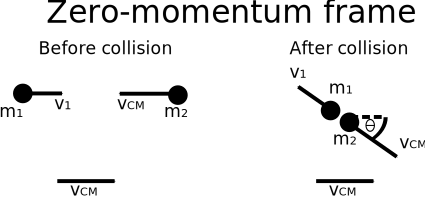
\includegraphics[scale =1]{dynamics_zero_momentum_frame_deflection}
\caption{}
\label{fig:dynamics_zero_momentum_frame_deflection}
\end{figure}


In the zero momentum frame, the speed of \vari{m_{1}} before the collision (through conservation of momentum) is given by $v_1 = \frac{m_{2}u}{m_{1} + m_{2}}$. After the collision, to ensure that the total momentum in the frame remains at zero, as well as conserving the energy of the system, both particles must be moving at the same speed as before the collision but travelling directly away from each other. However the angle \vari{\theta} shown in the diagram can take any value.


Translating this back into the lab frame gives of possible different velocities for mass  \vari{m_{1}}, which would each consist of a vector starting from the particle on the diagram and ending at a point on the circle of radius \vari{v_1} shown.

\begin{figure}[h]
\centering
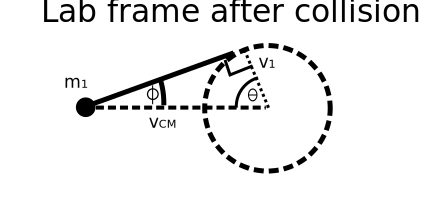
\includegraphics[scale =1]{dynamics_lab_frame_deflection}
\caption{}
\label{fig:dynamics_lab_frame_deflection}
\end{figure}

 The maximum deflection angle is obtained when the velocity of mass \vari{m_{1}} forms a tangent to this circle, giving a deflection angle \vari{\phi} obeying the equation $\sin{\phi} =  \frac{v_1}{v_CM} = \frac{m_2}{m_1}$ }% The solution text goes in the final bracket pair.
\end{problem}

